\chapter{Introduzione}
\section{Ripasso}
Nel percorso universitario affrontato fino a questo momento, sono state studiate
le basi di dati centralizzate, ovvero basi di dati in cui i dati sono memorizzati
in un unico luogo. L'architettura di tali strumenti è definita attraverso:
\begin{itemize}
      \item Uno o più spazi per la memorizzazione dei dati, tutti localizzati nello
            stesso luogo.
      \item Il DBMS, che è un software che consente di gestire i dati.
      \item Un'interfaccia che consente agli utenti di leggere e scrivere i dati.
\end{itemize}
\begin{definizione}[\textbf{DBMS}]
    Un \textbf{DBMS} (Database Management System) è un sistema software che
    consente di gestire in modo efficiente e sicuro grandi quantità di dati,
    garantendo la loro integrità e la loro disponibilità.

    Le collezioni di dati che vengono gestite da un DBMS sono:
    \begin{itemize}
          \item \textbf{Grandi}: ovvero di dimensioni maggiori rispetto a quelle
                che possono essere gestite da un singolo file.
          \item \textbf{Persistenti}: ovvero che hanno un periodo di vita
                indipendente da quello del programma che li utilizza.
          \item \textbf{Condivise}: ovvero che possono essere utilizzate da
                più utenti contemporaneamente, i quali possono accedere ai dati
                sia in lettura che in scrittura. Questo comporta la necessità di
                garantire la coerenza dei dati e di definire il workflow di accesso.
          \item \textbf{Affidabilità}: ovvero che devono essere garantite
                l'integrità e la disponibilità dei dati. Le transazioni devono
                essere atomiche, cioè o vengono eseguite completamente o non
                vengono eseguite affatto.
    \end{itemize}
\end{definizione}
Per quanto riguarda i DBMS, la loro architettura dati è definita su tre livelli:
\begin{enumerate}
      \item \textbf{Schema esterno}: rappresenta ciò che vede l'utente finale,
            permette all'utente di avere viste personalizzate dei dati.
      \item \textbf{Schema concettuale}: è la rappresentazione dei dati in modo
            indipendente dal DBMS. Questo schema è definito attraverso un modello
            di dati, che può essere relazionale, gerarchico, a oggetti, ecc.
      \item \textbf{Schema fisico}: questo schema rappresenta l'approccio fisico
            del sistema e quindi le modalità utilizzate da un DBMS per implementare
            le sue tabelle, le sue configurazioni, tutti i dati di cui ha bisogno
            sulla memoria fisica stessa.
\end{enumerate}
\begin{nota}
      Uno schema fisico è associato ad un solo schema concettuale.
\end{nota}
Inoltre, i DBMS centralizzati sono caratterizzati da:
\begin{itemize}
      \item Nessuna distribuzione dei dati e nessuna eterogeneità fisica.
      \item Un unico linguaggio di interrogazione.
      \item Un unico sistema di gestione di accesso ai dati.
      \item Un unica modalità di ripristino a fronte dei guasti.
      \item Un unico amministratore dei dati e quindi nessuna autonomia gestionale.
\end{itemize}
A causa degli accessi condivisi ai database si hanno problemi di \textbf{concorrenza},
avendo accesso multi-utente alla stessa dei dati condivisa. In merito alla
concorrenza si ha che le transazioni sono corrette se sono \textbf{seriali}
(ordinate temporalmente) ma questo non è sempre applicabile in quanto si vanno
ad aumentare i tempi per eseguire le operazioni, e quindi si deve stabilire un
controllo della concorrenza.

Inoltre, il controllo della concorrenza permette anche di garantire la
\textbf{consistenza} del sistema, ma a volte potrebbe essere più conveniente
prediligere la concorrenza piuttosto che la consistenza.

Un ulteriore problema di sicurezza è dato dalla \textbf{privacy}, ovvero la
necessità di garantire che i dati siano accessibili solo a chi ha i permessi
per farlo. Risulta quindi necessario introdurre un sistema di autenticazione
e autorizzazione.

\section{Gestione dei dati tramite Use Case}
Nella gestione dei dati non sempre è sufficiente un DB relazionale soprattutto
quando si hanno tanti dati e tanti utenti in accesso.

Nella gestione dobbiamo tenere traccia dei workload, carichi di lavoro che dipendono da:
\begin{itemize}
    \item letture/scritture
    \item numero di operazioni
    \item complessità delle operazioni
\end{itemize}
Un altro aspetto importante sono i volumi dei dati e l'eterogeneità.

Quando si trattano i dati si ha una pipeline di lavoro (value chain) composta da
tre fasi:
\begin{itemize}
    \item \textbf{Data discovery}: ottenimento, preparazione e organizzazione
          dei dati da diverse fonti
    \item \textbf{Data integration}: integrazione di tutti i dati provenienti da
          diverse fonti
    \item \textbf{data exploitation}: analisi dei dati, visualizzazione e presa
          di decisione (studio esplorativo).
\end{itemize}
Per queste operazioni esistono differenti prodotti.
% ! Immagine catena
L'obiettivo del corso è quello di progettare un'architettura dati in base al contesto.
Conoscere le tipologie di prodotti, nuovi modelli DBMS e gestione dei dati.

Tutto si basa sugli Use Case
\begin{itemize}
    \item \textbf{Caso Bancario}: un'architettura dati che permetta di effettuare 
          le normali operazioni bancarie. Questo consiste nella progettazione di 
          un sistema distribuito relazionale (diversi database distribuiti), che
          gestisce interrogazioni e transazioni distribuite.
    \item \textbf{Machine Learning}: realizzazione di una pipeline per la 
          costruzione dei dataset di training per addestrare modelli di ML. 
          DAta centric AI, MLops.
    \item \textbf{Modelli e architetture non relazionali}: ne sono un esempio le API
          che restituiscono dati in formato JSON. Comprendono quindi modelli key-value,
          grafi, sistemi distribuiti relazionali ecc...
    \item \textbf{Cloud}: Utilizzo di sistemi di gestione dei dati in cloud, firebase e elastic search.
    \item \textbf{AI generativa per la gestione dei dati}: come usare AI generativa nei 
          sistemi di gestione dei dati.
\end{itemize}

% Sistemo appena carica le slide
\section{Gestione operazioni bancarie}
Si vuole un'architettura dati che permetta di effettuare le normali operazioni
bancarie. Servirà la progettazione di sistemi distribuiti relazionali (diversi database distribuiti),
interrogazioni distribuite e transazioni distribuite.

Abbiamo le seguenti operazioni:
\begin{itemize}
    \item transizioni bancarie
    \item bonifici multibanca
\end{itemize}

Per prima cosa bisogna studiare il workload:
\begin{itemize}
    \item letture e scritture: bilanciate
    \item quante sono: sono tante
    \item complessità: semplici
\end{itemize}

I volume dei dati è elevato

Si ha eterogeneità dei sistemi.

Bisogna stare attenti agli update che devono essere veloci e consistenti. L'architettura
di base non è più sufficiente.

\begin{figure}[ht]
      \centering
      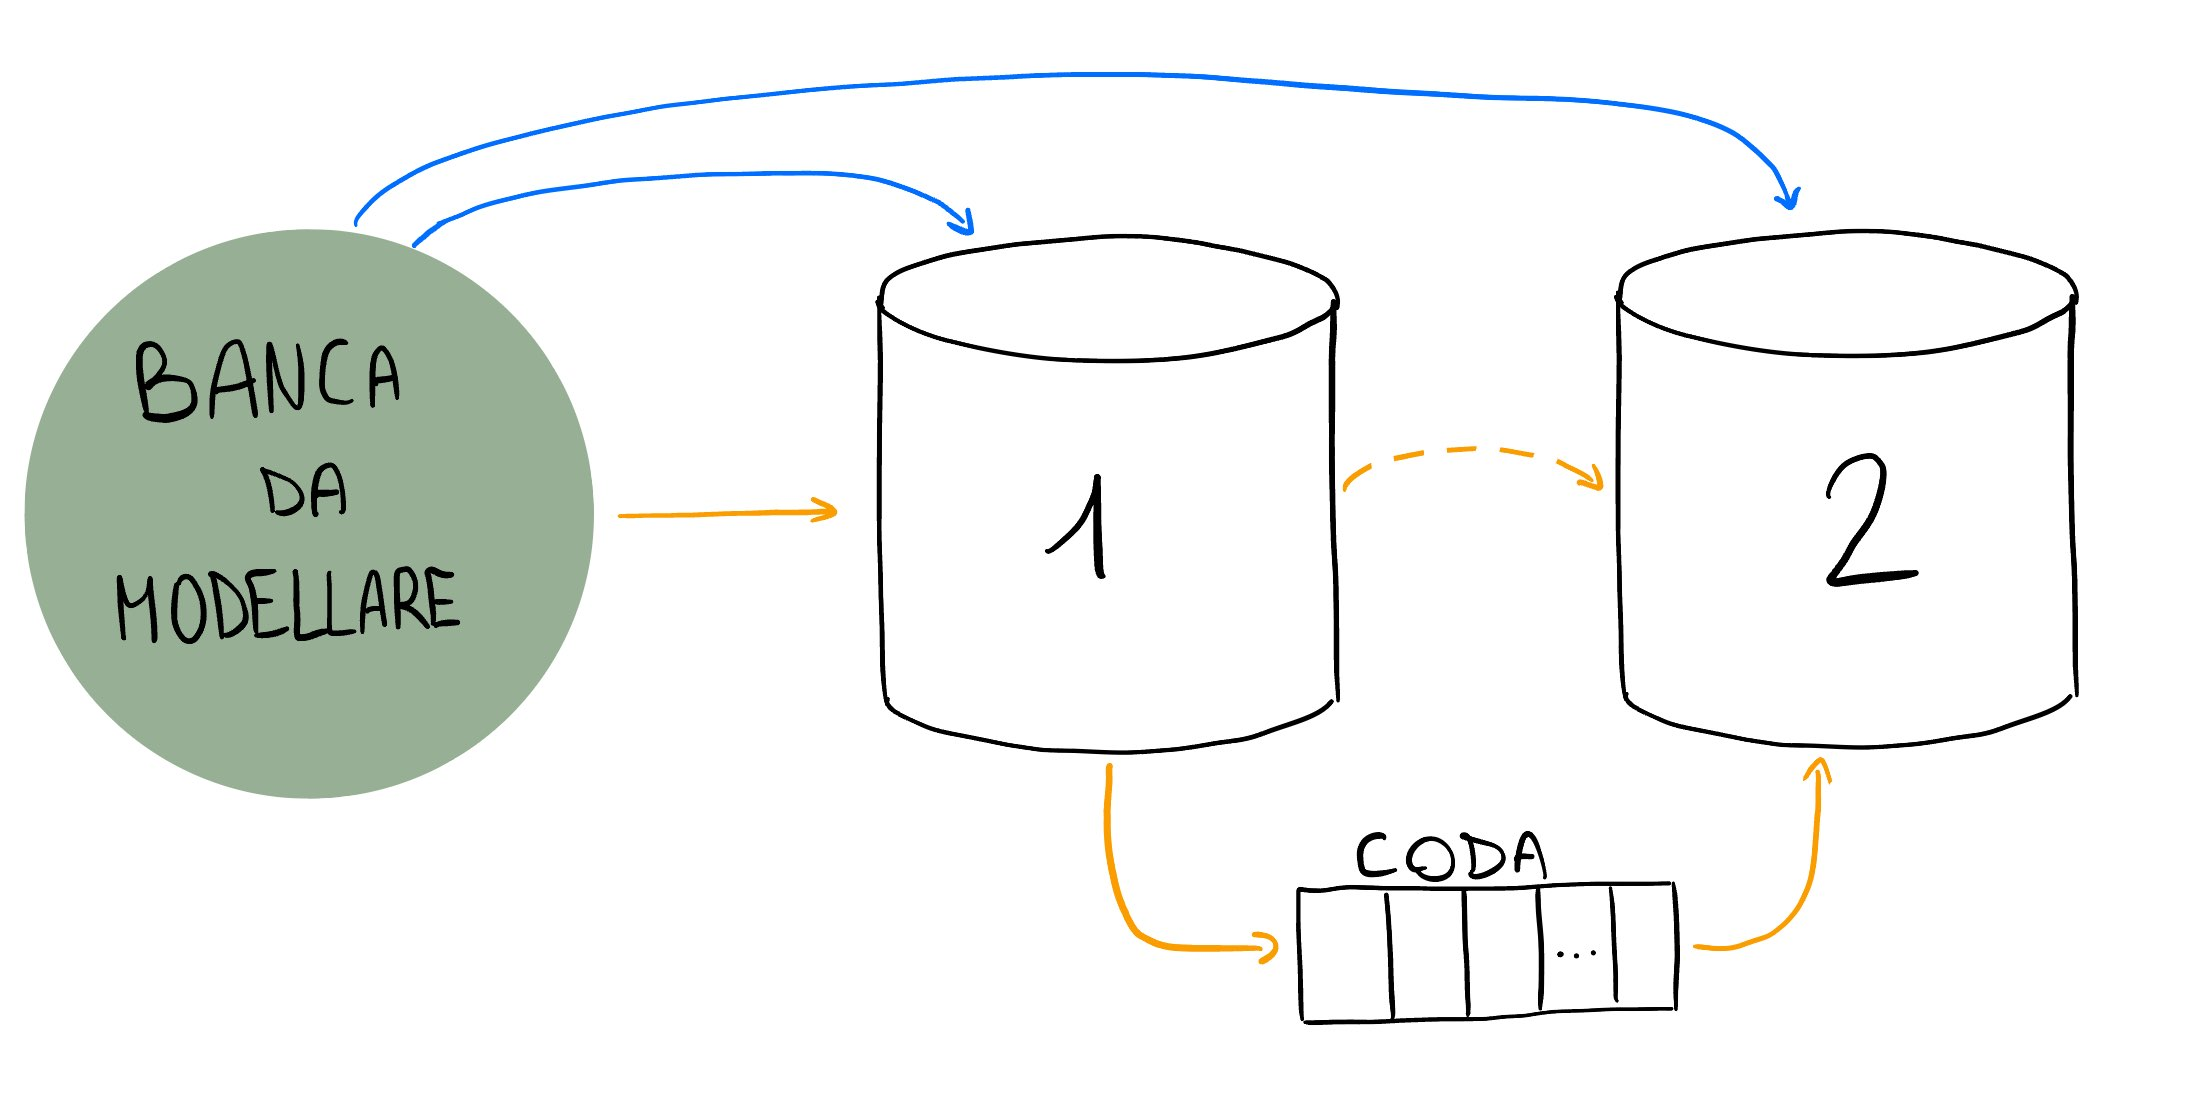
\includegraphics[width=0.8\textwidth]{./img/modellazione_banca.jpg}
      \caption{Architettura dati per update veloci e consistenti}
\end{figure}

Bisogni:
\begin{itemize}
    \item Persistenza dei dati: replica dei dati attraverso un Master Slave. Per
          gestire la replica e il continuo dei servizi ho bisogno di un middleware che
          permette di mantenere la consistenza tra le due istanze. Nota: distribuire
          i dati è molto complesso e rischioso, conviene farlo solo quando è davvero
          necessario prima di aggiungere complessità inutilmente. Motori di database
          distribuiti, frammentare i dati tra nodi diversi, oppure edge computing i device
          salvano localmente i dati. Il problema è che quando si distribuiscono i dati
          bisogna capire cosa distribuire, ovvero capire come distribuire tra client e
          server le parti di gestione.
\end{itemize}

Possiamo avere 3 sedi dislocate geograficamente, il nodo di Milano ha la logica applicativa
e i dati mentre a Roma e Padova ho solo l'applicazione. Si possono frammentare i
dati in modo da portarli vicino a dove servono, ex: Roma c'è il reparto risorse
umane allora i dati sulle risorse umane verranno spostati lì. Spesso nella frammentazione
si hanno dati in comune tra due sedi, quindi si effettuerà anche una duplicazione
dei dati (replica).
